\PassOptionsToPackage{dvipsnames}{xcolor}

\documentclass[a4paper,12pt]{book}
\usepackage[titletoc]{appendix}
\usepackage{amsmath}
\usepackage{float}
\usepackage{tabularx}
\usepackage{amssymb}
\usepackage{amsthm}
\usepackage{xspace}
\usepackage{listings}
\usepackage{indentfirst}
\usepackage{fancyhdr}
\usepackage{multicol}
\lstset{
	frame=single,
	breaklines=true,
	postbreak=\raisebox{0ex}[0ex][0ex]{\ensuremath{\color{red}\hookrightarrow\space}},
	numbers=left,
	stepnumber=1,    
	firstnumber=1,
	numberfirstline=true,
    showstringspaces=false,
    upquote=true,
    literate={``}{\textquotedblleft}1
}
\usepackage{multirow}

\usepackage[dvipsnames,svgnames,x11names]{xcolor}
\usepackage[markup=underlined]{changes}
\definechangesauthor[color=BrickRed]{PRH}
\definechangesauthor[color=NavyBlue]{RPA}
\definechangesauthor[color=Green]{MJV}

\usepackage{todonotes}
\setlength{\marginparwidth}{2.4cm}
\makeatletter
%\setremarkmarkup{\todo[color=Changes@Color#1!20,size=\scriptsize]{#1: #2}}
\makeatother
%% Rather hacky definition of a plain remark/note
%% by riding on \added
\newcommand{\note}[2][]{\added[#1,remark={#2}]{}}


\usepackage{hyperref}
\usepackage{array}
%\usepackage[breaklinks]{hyperref}
%\usepackage[portuguese]{babel}
\usepackage[utf8]{inputenc}
\usepackage{graphicx}
\usepackage{fancyhdr}
\usepackage{acronym}
\usepackage{tocvsec2}
\usepackage{enumerate}
\usepackage{scalefnt}
%\usepackage{calc}
\usepackage{setspace}
\usepackage{color,colortbl,multirow}
%\usepackage{longtable}
\usepackage{pgfgantt}
\usepackage{xcolor}
\usepackage{tikz}
\usepackage{rotating}
\usepackage{pdflscape}
\usepackage{tabulary}
\usepackage{array}
\usepackage{arydshln}
\usepackage{natbib}
\usepackage{caption}
\usepackage{booktabs}
\usepackage{lscape}
\usepackage{verbatim}
\usepackage{fancyvrb}
%pacote de colocar second
\usepackage[super]{nth}
%\DeclareMathOperator*{\Max}{Max}
%\DeclareMathOperator*{\Min}{Min}
\definecolor{cinzaclaro}{gray}{0.9}
\definecolor{preto}{gray}{1}
%\def\tm{\leavevmode\hbox{$\rm {}^{TM}$}}

\usepackage[hang,multiple]{footmisc}
\renewcommand{\footnotelayout}{\raggedright}

% corrigir margens 
\oddsidemargin 2cm
\evensidemargin 0.5cm

\usepackage{listingsutf8}
\lstset{
	frame=single,
	breaklines=true,
	postbreak=\raisebox{0ex}[0ex][0ex]{\ensuremath{\color{red}\hookrightarrow\space}}
}

%Cabe�alho

\pagestyle{fancy}
%\fancyheadoffset[LE,RO]{1cm}
\renewcommand{\chaptermark}[1]{\markboth{#1}{}}
\renewcommand{\sectionmark}[1]{\markright{\thesection\ #1}}
\fancypagestyle{normal}{%
	\fancyheadoffset[LE,RO]{1cm}
	\fancyhf{}
   	\fancyhead{} % clean header   	
   	\fancyfoot{}
	\fancyhead[LE,RO]{\bfseries\thepage}
	\fancyhead[LO]{\bfseries\rightmark}
	\fancyhead[RE]{\bfseries\leftmark}
	\renewcommand{\headrulewidth}{0.5pt}
}

\fancypagestyle{empty}{%
   	\fancyhead{} % clean header   	
   	\fancyfoot{}
   	\renewcommand{\headrulewidth}{0pt} % and the line
}

\fancypagestyle{footer}{%
	\fancyhead{}
	\renewcommand{\headrulewidth}{0pt}
   	\fancyfoot[C]{\bfseries\thepage} % clean header   		
}


%ABSTRACT - Added at January 8
\newcommand\abstractname{Abstract}  %%% here
\makeatletter
\if@titlepage
  \newenvironment{abstract}{%
      \titlepage
      \null\vfil
      \@beginparpenalty\@lowpenalty
      %\begin{center}%
        %\bfseries
        {\Large\textbf{\abstractname}}
        \@endparpenalty\@M
      %\end{center}
      }%
     {\par\vfil\null\endtitlepage}
\else
  \newenvironment{abstract}{%
      \if@twocolumn
        {\Large\textbf{\section*{\abstractname}}}%
      \else
        \small
        %\begin{center}%
          {%\bfseries
          {\Large\abstractname\vspace{-.5em}\vspace{\z@}}}%
        %\end{center}%
        \quotation
      \fi}
      {\if@twocolumn\else\endquotation\fi}
\fi
\makeatother 
%ABSTRACT
 
\begin{document}

\makeatletter
\newcommand{\rmnum}[1]{\romannumeral #1}
\newcommand{\Rmnum}[1]{\expandafter\@slowromancap\romannumeral #1@}
\makeatother

% Code for creating empty pages
%No headers on empty pages before new chapter
\makeatletter
\def\cleardoublepage{\clearpage\if@twoside \ifodd\c@page\else
    \hbox{}
    \thispagestyle{empty}
    \newpage
    \if@twocolumn\hbox{}\newpage\fi\fi}
\makeatother \clearpage{\pagestyle{normal}\cleardoublepage}

\raggedbottom 

\begin{titlepage}
\vspace{\stretch{1}}
\begin{center}
 
\includegraphics[scale=1]{images/EENG.jpg}
 \end{center}
\begin{center}
\color[gray]{0.5}Escola de Engenharia

\end{center}
\begin{minipage}[!b]{\textwidth}
\vspace{5cm}
\begin{flushleft}
\color[gray]{0.5}{\Large Applying Attribute Grammars to teach Linguistic Rules}\\
\vspace{2cm}
\begin{large}
\textbf{Manuel Gouveia Carneiro de Sousa}\\
%\url{manuelgcsousa@gmail.com}\\
\end{large}
\vspace{1cm}
\color[gray]{0.5}Supervisor:\\
\color[gray]{0.3}\textbf{Ph.D Pedro Manuel Rangel Santos Henriques}\\
\color[gray]{0.4}Co-supervisor:\\
\color[gray]{0.3}\textbf{Ph.D Maria João T. Varanda Pereira}\\
\vspace{0.3cm}

\vspace{3cm}
\end{flushleft}
\centering \today

\end{minipage}

\end{titlepage}
\newpage
\cleardoublepage

\begin{center}
    \textbf{AUTHOR COPYRIGHTS AND TERMS OF USAGE BY THIRD PARTIES}
\end{center}
        
This is an academic work which can be utilized by third parties given that the rules and good practices internationally accepted, regarding author copyrights and related copyrights.

Therefore, the present work can be utilized according to the terms provided in the license bellow.

If the user needs permission to use the work in conditions not foreseen by the licensing indicated, the user should contact the author, through the RepositóriUM of University of Minho.\\[0.5cm]

\textbf{License provided to the users of this work}


\includegraphics[width=0.2\textwidth]{images/license.png}

\textbf{Attribution-NonCommercial}

\textbf{CC BY-NC}

https://creativecommons.org/licenses/by-nc/4.0/

\newpage

\begin{center}
    \textbf{STATEMENT OF INTEGRITY}
\end{center}

I hereby declare having conducted this academic work with integrity. I confirm that I have not used plagiarism or any form of undue use of information or falsification of results along the process leading to its elaboration.

I further declare that I have fully acknowledged the Code of Ethical Conduct of the University of Minho.\\[0.5cm]

\begin{flushright}
\begin{tabular}{@{}p{1.2in}}
Manuel Sousa \\
\hrulefill \\
\end{tabular}
\end{flushright}
% paragraf indentation
\setlength{\parindent}{1.5pt}
\setlength{\parskip}{1.5ex plus 0.5ex minus 0.2ex}
\onehalfspacing

\pagenumbering{roman}
%\input{chapters/0_resumo}
%\cleardoublepage
\pagestyle{footer}

\begin{titlepage}
\renewcommand{\abstractname}{\vspace{-\baselineskip}}

% english
\begin{abstract}
\section*{Abstract}

This document presents a proposal for a Master Thesis within the topic of “Applying Attribute Grammars to teach Linguistic Rules”, and will be accomplished at Universidade do Minho in Braga, Portugal.

\noindent This thesis is focused on using the formalisms of attribute grammars in order to create a tool to help linguistic students learn the different rules of a natural language. The main goal is to create a new \textsc{DSL} with a simple notation, suitable for any person that does not have any experience with common programming languages elements. Furthermore, it is expected to create a user interface that supports that same tool, granting a more visual experience for the user.\\[0.1cm]
    
\noindent \textbf{Keywords}: Linguistic, Natural Language, Attribute Grammars

\end{abstract}

%%%%%%%%%%%%%%%%%%%%%%%%%%%%%%%%%%%%%%%%%%%%%%%%%%%%%%%%%%%%%%%%%%%%%%%%%%%%%%%%%%%%%%%%%%%%%%%%%%%%%%%%

% portuguese
\begin{abstract}
\section*{Resumo}

Este documento refere-se a uma dissertação sobre o tópico ``Aplicar Gramáticas de Atributos no ensino de Regras de Linguística'', e será concluída na Universidade do Minho em Braga, Portugal.
	
\noindent Esta dissertação pretende focar-se no uso dos formalismos das gramáticas de atributos de maneira a criar uma ferramenta que ajude os alunos de linguística a aprender as diversas regras da língua natural. O principal objetivo é a criação de uma \textsc{DSL} com uma notação simples, adequada a qualquer pessoa que não tenha experiência com elementos comuns das linguagens de programação. Para além disso, é esperada a criação de uma interface que sirva de suporte a essa mesma ferramenta, permitindo assim uma experiência visual ao utilizador.\\[0.1cm]
    
\noindent \textbf{Palavras-chave}: Linguística, Língua Natural, Gramáticas de Atributos

\end{abstract}

\end{titlepage}
\setlength{\parindent}{1.5pt}
\setlength{\parskip}{0pt}
\singlespacing

% paragraf indentation
\setlength{\parindent}{1.5pt}
\setlength{\parskip}{0pt}

% % Table of Contents
\settocdepth{subsection}
\tableofcontents
\pagebreak

\listoffigures
\addcontentsline{toc}{chapter}{List of Figures}
\pagebreak

\listoftables
\addcontentsline{toc}{chapter}{List of Tables}
\pagebreak

% % ABBREVIATIONS

\chapter*{List of Acronyms}
\addcontentsline{toc}{chapter}{List of Acronyms}

\begin{tabular}{ll}

DSL   & Domain Specific Language\\[0.1cm]
ANTLR & Another Tool for Language Recognition\\[0.1cm]
CFG   & Context-free Grammar\\[0.1cm]
AG    & Attribute Grammar\\[0.1cm]

\end{tabular}



\cleardoublepage
\pagestyle{normal}
% reset to arabic again
\pagenumbering{arabic}

% paragraf indentation
\setlength{\parindent}{1.5pt}
\setlength{\parskip}{1.5ex plus 0.5ex minus 0.2ex}
\onehalfspacing


%\addcontentsline{toc}{chapter}{Introduction}
\pagestyle{normal}
\setlength{\parindent}{1.5cm}
\setlength{\parskip}{1.5ex plus 0.5ex minus 0.2ex}
\chapter{Introduction} \label{introduction}
	
\section{Context}
Attribute Grammars are a way of specifying syntax and semantics to describe formal languages \cite{hafiz_2011} and were first developed by the computer scientist Donald Knuth in order to formalize the semantics of a context-free language \cite{slonneger_1995}. They were created and are still used for language developing, compiler generation, algorithm design, etc \cite{thirunarayan_2009}. One other application would be the teaching of linguistic rules through the usage of formalisms presented in attribute grammars \cite{horakova_2014}. Using attribute grammars, it is possible to specify the way sentences are correctly written. By making use of ``synthesized attributes'', it would be possible to represent the gender of an adjective, while ``inherited attributes'' would be translated into the meaning of a preposition, depending on the context of the sentence \cite{donald_1990}.
There are an array of linguistic rules to be represented within an attribute grammar, and when a sentence is provided, it is possible to validate the syntax, adverting for any errors that may be encountered \cite{barros_2017}.

Applying attribute grammars to model all the different syntax and semantic behaviour of natural languages is a technique that has already been practiced, but it demands knowledge in programming syntax in order to translate natural languages rules to attribute grammar rules \cite{hafiz_2011}. In spite of the existing tools, they are not so easily available and straightforward for those who do not have programming and computation proficiency - in this specific case, linguists. There are tools available that use languages which closely resembles logic, and use logic components, but it is easier to rapidly grasp the concepts of a domain specific language, that only does a list of tasks, than to use a language that is not created with a main purpose.
    
So, the main proposal is to define a new \textsc{DSL} (Domain Specific Language) with a much simpler notation, making it easy to learn and to rapidly understand. The main focus is to keep the syntax as close as possible to a natural language, avoiding common programming languages elements (such as semicolons, curly brackets, etc.). This allows the specification of rules to be done in a much natural manner. Also, it is desired to create a visually appealing user interface, granting the user the possibility of analysing the generated syntax-tree.

	
\section{Objective}
The main objective of this master thesis is to produce a pedagogical tool to support teaching linguistics. The detailed objetives are the following:

\begin{itemize}
    \item Definition of simple and concise \textsc{DSL}, suitable for common users, to specify linguistic rules based in an attribute grammar.
    \item Construction of that pedagogical tool, with a friendly user interface, based on the reffered attribute grammar using \textsc{ANTLR} (ANother Tool for Language Recognition).
\end{itemize}
    
\section{Methodology}
The research work will be performed at different stages. The methodology that will be followed to achieve this master project will focus on literature revision, solution proposal, implementation and testing. The following steps realise this methodology:

\begin{itemize}
    \item Do a comprehensive research about attribute grammars in linguistics: what has been done, how has it been done, and ways to improve the previous work.
    \item Research the principles of linguistic rules in different languages.
    \item Design a \textsc{DSL} that allows a straightforward specification of an array of rules.
    \item Develop a language translator that can translate programs written in the new language to \textsc{ANTLR}.
    \item Create an user interface that allows for a visual analysis of the generated syntax-tree.
    \item Experiment with some case studies, and test the tool with real linguistic students.
\end{itemize}
    
\section{Document Structure}
The document starts by introducing the problem, and in \textbf{Chapter 1} a context, objectives and methodology are presented.
On \textbf{Chapter 2} the main concepts are briefly explained, followed by the presentation and explanation of current existing solutions that may help solving the current problem.
\textbf{Chapter 3} consists on explaining the proposal for solving the stated problem, documenting the system architecture, giving some examples and then using the tool produced.
\textbf{Chapter 4} intends to close the document with summary of the work that was done, opinions on what was done, and explains what are the next steps to take in order to achieve the main objective.
\chapter{State of the art} \label{state_of_the_art}

In this chapter is of the utmost importance to define some concepts that were used has a basis for this thesis. in addition, it will be discussed possible tools that already answer some of the questions that this thesis is trying to answer, and for that matter are important to be studied and referenced.
	
\section{Domain Specific Language}
A domain specific language is an ``executable specification language, through appropriate notations and abstractions'', usually restricted to a particular problem domain. Their objective is to improve productivity, and to allow solutions to be expressed in the idiom and at the level of abstraction of the problem domain \cite{van_2000}.
	
This types of languages provide a natural vocabulary for concepts that are fundamental to the problem scope \cite{bruce_1997}, something that may lack when using a general-purpose language. \textsc{DSLs} are usually small and declarative, with very specific goals \cite{van_2000}. Refered as ``little languages'' \cite{bentley_1986}, they are intended to solve problems within a specific domain, and not outside it.
	
\section{Attribute Grammar}
Attribute Grammars were proposed by Donald Knuth in order to specify static and dynamic semantics of a programming language in a syntax-directed manner \cite{thirunarayan_2009}. The process consists in constructing the syntax tree and then computing the values of attributes by visiting every single node. For each attribute it is possible to associate a domain of values, such as integers, strings or even complex structures. Formally an attribute grammar (AG) is a tuple \cite{pereira_2016}
	
\begin{description}
    AG = \textless CFG, A, CR, CC, TR\textgreater
\end{description}
that is composed by a context-free grammar (CFG), that has been extended to provide context by using a set of attributes; Those same set of attributes (A), which exist in each production of a grammar, and are divided into two groups, \emph{Synthezized Attributes}, which allows values to be pass one from a node to its parent, and \emph{Inherited Attributes}, which allows values to be pass on from the current node to a child \cite{slonneger_1995}; rules for calculating attributes (CR) in all productions of the grammar; a set of contextual conditions (CC); and the transformation rules (TR) in all productions of the grammar.

\section{PAG  (Prototyping with Attribute Grammars)}
PAG is a tool that was created with the purpose of helping two distinct groups of students from \emph{Universidad Complutense de Madrid}. One of those groups, involving computer science students, that attended a class which teached compiler contructions, and other group involving linguistic students, with a class on computacional linguistics. Teachers from both classes used the same methodology to teach their classes, na dnoticed that it wasnt good enough for the students to master all the concepts: On one hand, they would have computer science skilled students, with great apititude to produce solutions, but leaving aside the respective specifications, which lead to poor and innacurate formal specifications, but on the other hand, linguistic students produced good formal specifications, as they are proficient with the natural language, but lack computer science skills to well transpose all the knowledge into computacional models \cite{sierra_2006}.
	
The result was an environment based in attribute grammars that allows the specification of those same grammars using a language close to Prolog. The main goal was to embed Prolog into the language and maintain all the familiar basic notation, the reason being both groups of students were already familiar with the Prolog and attribute grammar syntax and notation. Through rapid prototyping, which PAG makes use of, it is possible to obtain a functional processor at a embryonic state of the problem \cite{sierra_2006}. With this, computer science students can obtain results quite early, allowing them to apply more time into formal specifications. Moreoever, as the complexity of the syntax is reduced, this allows for a better and easier learning experience for students which have less aptitude for the solution codification or programming in general, which is the case for linguistic students.
	
Overall, PAG solved the problem that was purposed in an effective way. Despite that, and giving the respective credit to the those who built the tool, the fact is that Prolog can still be quite difficult to grasp for some people, and a challenge when it comes to learn it. The usage of a specification language that closely resembles the natural one, could be a great addition.
	
\section{VisualLISA (A Visual Programming Environment for Attribute Grammars)}
VisualLISA is a visual programming environment created by Pedro Oliveira in the year of 2009 \cite{oliveira_2009} for the specification of attribute grammars. Classified as a ``Domain Specific  Visual Language'', its main goal was to enhance the front-end of one other tool named LISA \footnote{https://labraj.feri.um.si/lisa/}, a compiler generator based in AG's that creates different visual tools based on the textual specification of the grammars.
    
The aim of this tool was to decrease the difficulty which is involved with specifying attribute grammars, not only for the LISA environment, but also regarding other types of systems, making specifications more visual and graphical.
    
Specifying grammars in a visual manner can be done using a set of icons (\autoref{fig:visuallisa_icons}) that must be combined to obtain the wanted result. Each icon or symbol has a unique function, and it is the users task to make the connections in a correct way.
    
% Imagem dos icons do VisualLISA
\begin{figure}[h]
    \centering
    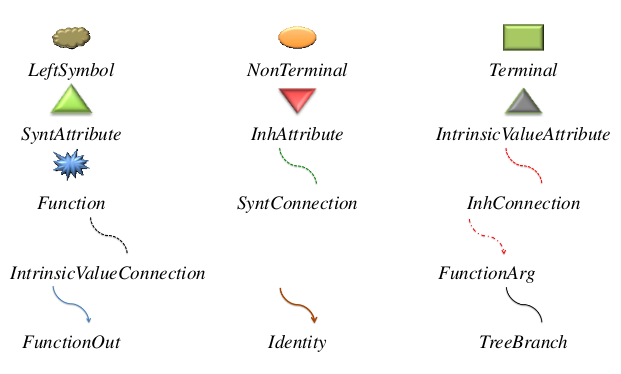
\includegraphics[width=10cm]{images/visuallisa_icons.png}
    \caption{VisualLISA set of icons.}
    \label{fig:visuallisa_icons}
\end{figure}
    
The environment (\autoref{fig:visuallisa_window}) consists in 4 windows, each one with an individual task: declare the productions of the grammar in a textual manner; declare functions, data-types, etc. ; draw the grammar productions; specify computation rules that were previously declared.
    
% Imagem da janela do VisualLISA
\begin{figure}[h]
    \centering
    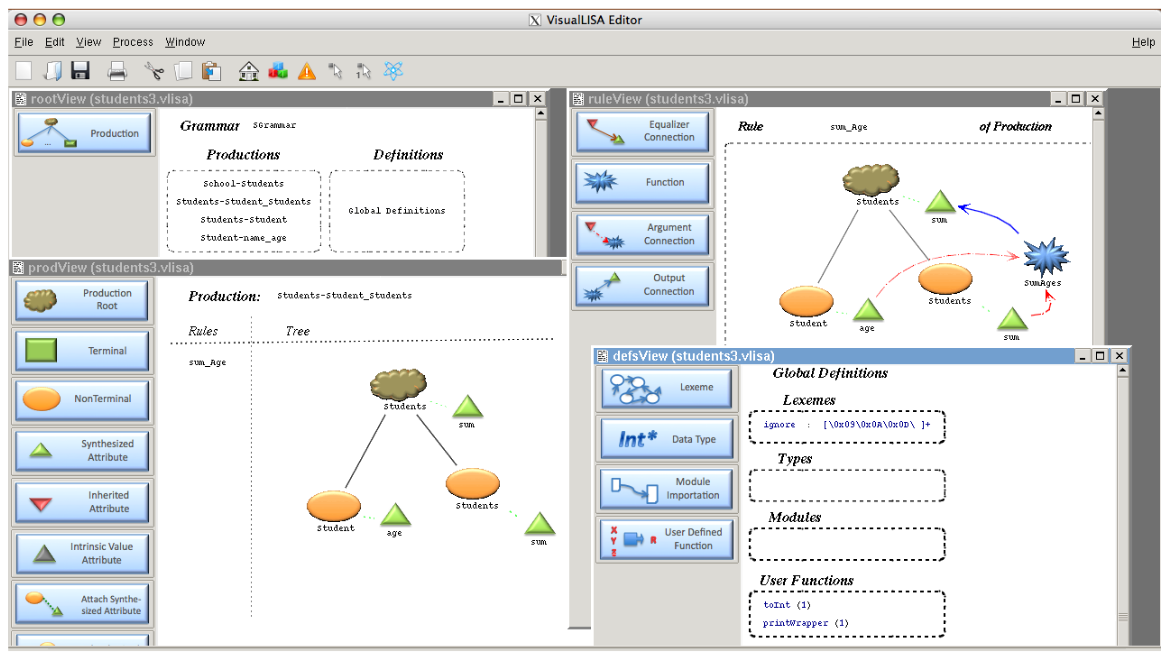
\includegraphics[width=10cm]{images/visuallisa_window.png}
    \caption{VisualLISA main window.}
    \label{fig:visuallisa_window}
\end{figure}
    
As an example, it was included a textual specification (\autoref{fig:textual_students_grammar}) and the respective graphical specification (\autoref{fig:graphical_students_grammar}), extracted from the proper article \cite{oliveira_2009}.
    
% Students Grammar
\begin{figure}[h]
    \centering
    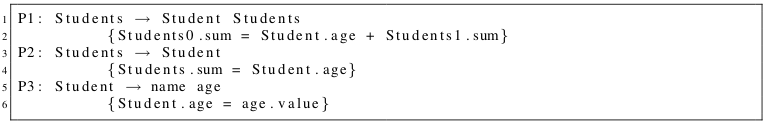
\includegraphics[width=15cm]{images/textual_students_grammar.png}
    \caption{Students textual grammar.}
    \label{fig:textual_students_grammar}
\end{figure}
    
% VisualLISA Conception
\begin{figure}[h]
    \centering
    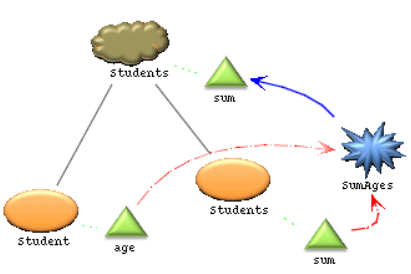
\includegraphics[width=8cm]{images/graphical_students_grammar.png}
    \caption{Students graphical grammar.}
    \label{fig:graphical_students_grammar}
\end{figure}

The main effect of the tool is not directly related to the problem that is trying to be solved, what is useful are all the visual components that are associated with it, which could help when creating the intended user interface for the visual analysis of the generated syntax-tree, or more. Nevertheless, it is a very useful and interesting way of aproaching attribute grammars and their specifications.
\chapter{Proposal} \label{proposal}

The main purpose of this proposal is the definition of a \textsc{DSL} that allows the specification of all different kinds of sentences, and afterwards, the possibility of testing given sentences as input and check if they are written accordingly to the rules previously specified. One obstacle that was encountered was how to extract the lexical part of the sentence, and in what way would each component be classified. In fact, this task is quite subjective, as different components may have various definitions in one context. % for example: (...). % Introduzir exemplo da professora!!!! 
Having known this, the decision was made that the student would beforehand identify the lexical part of the sentence.
% FALAR DO QUE VOU FAZER DE DIFERENTE (DICA DO LÁZARO!)

\section{System Architecture}
In order to specify all kinds of sentences/rules possible, the idea of creating a ``meta-language'' emerged. This ``meta-language'' is suppost to be the language in which the teacher would specify the rules for sentence construction. These rules would be written (in a single file) according to the following structure, that is divided into three main categories:

\begin{enumerate}
    \item \textbf{STRUCTURE} - this would be the block where the teacher would write how was the sentence suppost to be written, and what components would it have.
    
    \item \textbf{ERRORS} - list of conditions that the teacher would write in order to be analysed afterwards, for example, certain values for different attributes. If one of the conditions was matched, an error would appear.
    
    \item \textbf{INPUT} - this block corresponds to the ``parsing'' of the sentence (the lexical part) that the student wants to test. This would be written by the student and then automatically joined with the teachers information.
\end{enumerate}

This file would then be processed by an \textsc{ANTLR} processor that would work on the information that was written, and then generate a grammar (also specified in \textsc{ANTLR}). This grammar corresponds to the translation of the ``meta-language'' into \textsc{ANTLR} instructions. Afterwards, the generated grammar would be used to create a validator of sentences, where the student could write his sentence/sentences and obtain results. These results would be the validation of the given sentence/sentences and a tree for a better visualization of the input structure.

% Imagem da arquitetura do sistema.
\begin{figure}[h]
    \centering
    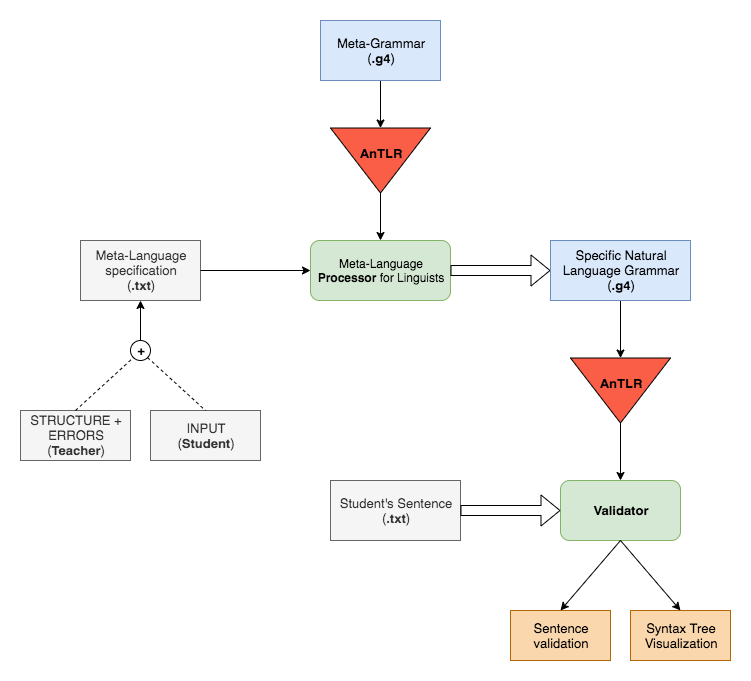
\includegraphics[width=12cm]{images/msc_system_architecture.png}
    \caption{System architecture.}
    \label{fig:system_architecture}
\end{figure}

\section{Meta-Language}
As it was stated in the beginning of this document, the main goal was to create a \textsc{DSL} that was easy to learn and to rapidly understand and grasp. With this in mind, the structure mencioned before on the first section of this chapter was followed: Three main parts, where two of them would be constructed by the teacher, and the third one was intended to be written by the student and later concatenated in a single file.

\subsection{Domain Specific Meta-Grammar}
The main intention of this language is to preprocess the information written by the teacher + student and then generate a validator for a particular structure. With simplicity in mind, a first version of the \textsc{DSL} was created, and it will be explained next.

\begin{figure}[h]
    \centering
    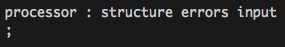
\includegraphics[width=7cm]{images/META_processor.png}
    \caption{DSL processor production.}
    \label{fig:dsl_processor_production}
\end{figure}

Firstly, the teacher specification will be discussed - meaning the \textbf{structure} and \textbf{errors} blocks.
The \textbf{structure} block is divided into \textbf{parts}, or main parts. These main parts correspond to the main components of the sentence. Each of these parts have an \textbf{element} within, containing the information about a certain component.

\begin{figure}[h]
    \centering
    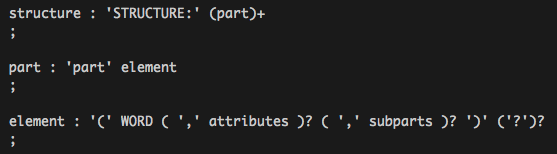
\includegraphics[width=10cm]{images/META_structure.png}
    \caption{DSL structure/part/element productions.}
    \label{fig:dsl_structure_production}
\end{figure}

The \textbf{element} is composed by the name of the component, a possible set of \textbf{attributes} and possible \textbf{subparts}.

\begin{figure}[h]
    \centering
    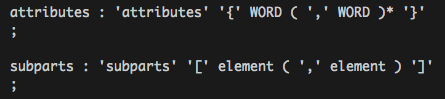
\includegraphics[width=8cm]{images/META_attributes_subparts.png}
    \caption{DSL attributes/subparts productions.}
    \label{fig:dsl_attributes_production}
\end{figure}

The \textbf{subparts} production intends to be the path for ``injecting'' more elements inside a single component. One component may be composed by several other components. As shown in the example above, the \textbf{subparts} production is a list of one or more elements.

Secondly, the teacher can define a list of restrictions to be applied to each attribute defined in the previous structure. These restrictions are logical conditions that must be obey for a sentence to be valid based on a specific structure.

\begin{figure}[h]
    \centering
    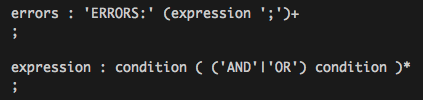
\includegraphics[width=8cm]{images/META_errors.png}
    \caption{DSL errors/expression productions.}
    \label{fig:dsl_errors_production}
\end{figure}

The \textbf{expression} production is a set of conditions that can be joined using the logical operators 'AND' and 'OR'. Each condition intends to access each attribute of any component and then assign it a value.

\begin{figure}[h]
    \centering
    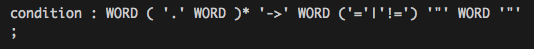
\includegraphics[width=10cm]{images/META_condition.png}
    \caption{DSL condition production.}
    \label{fig:dsl_condition_production}
\end{figure}

If, for instance, the teacher says that an attribute is equal to some value, then the student can not use said value with said attribute - this would result in an error.

Thirdly, and finally, the \textbf{input} block, which corresponds to the students section. This was treated has a different and separate \textsc{DSL}, as its main purpose was to identify the lexical parts of the sentence written by the student, allowing for a correct and non-subjective parsing of each word in the sentence. It is also important to notice that this first sketch is still \underline{verbose}, with only functionality in mind. By being treated as a separate \textsc{DSL}, it is accessible when it comes to changes, and simple to produce them.

\begin{figure}[h]
    \centering
    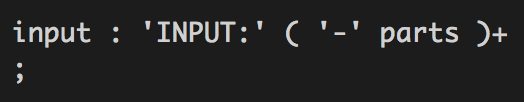
\includegraphics[width=7cm]{images/META_input.png}
    \caption{DSL input production.}
    \label{fig:dsl_input_production}
\end{figure}

The sketch starts within a section named \textbf{parts}, which corresponds to one sentence in particular. This production is composed by one or more blocks, where all the information is stored. Inside, the name of the components and their required attributes must be specified. It is also important to notice that a correct path must be specified by the student. If the student specifies a component that is not declared in the structure defined previously by the teacher, then an error should be thrown.

\begin{figure}[h]
    \centering
    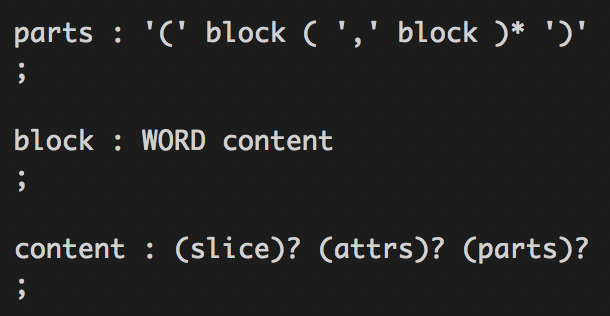
\includegraphics[width=8cm]{images/META_parts.png}
    \caption{DSL parts/component/content production.}
    \label{fig:dsl_parts_production}
\end{figure}

The student can specify the \textbf{slice} of the sentence that corresponds to the component that is being declared, and a set of attributes (\textbf{attrs}) that composes said component. Furthermore, it is possible to continue to define more \textbf{parts} within one part, just like the teacher's \textsc{DSL} \textbf{subparts}.

\begin{figure}[h]
    \centering
    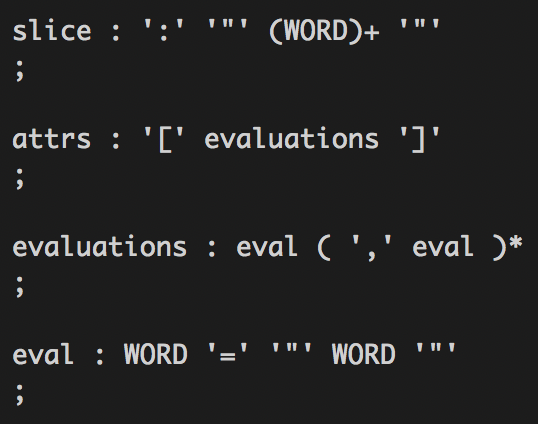
\includegraphics[width=8cm]{images/META_slice_attrs.png}
    \caption{DSL slice/attrs/evaluations/eval production.}
    \label{fig:dsl_slice_production}
\end{figure}

Inside the \textbf{slice} production, a list of words can be written. These are the words that will then be used to build the lexical part of the generated grammar. Also, when specifying attributes, the student must assign a value for each attribute that will then be used to validate each component of the sentence.

For a better understanding of the three main categories (structure, errors and input), bellow there is an example that is based on the first case study, and shows what the semantic of the teacher should look like.

% Exemplo de frase da meta gramática (parte do professor)
\begin{figure}[h]
    \centering
    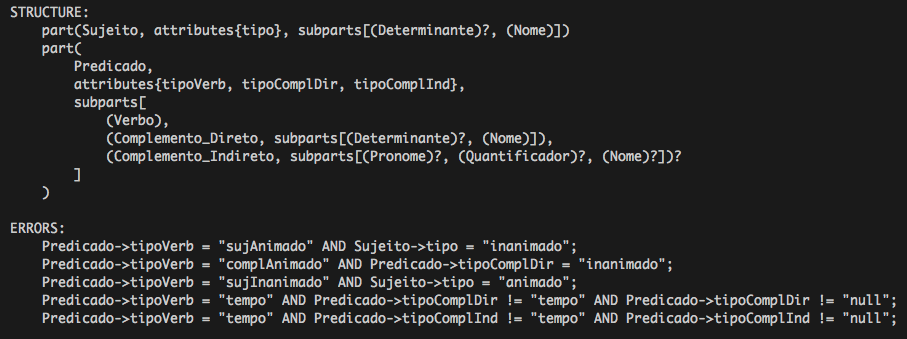
\includegraphics[width=15cm]{images/phrase_meta_grammar.png}
    \caption{Example of a possible sentence structure.}
    \label{fig:meta_grammar_teacher}
\end{figure}

In the case of the student, this is the semantic that should be used and one of the many examples that fit into the defined structured.

% Exemplo de frase da meta gramática (parte do aluno)
\begin{figure}[h]
    \centering
    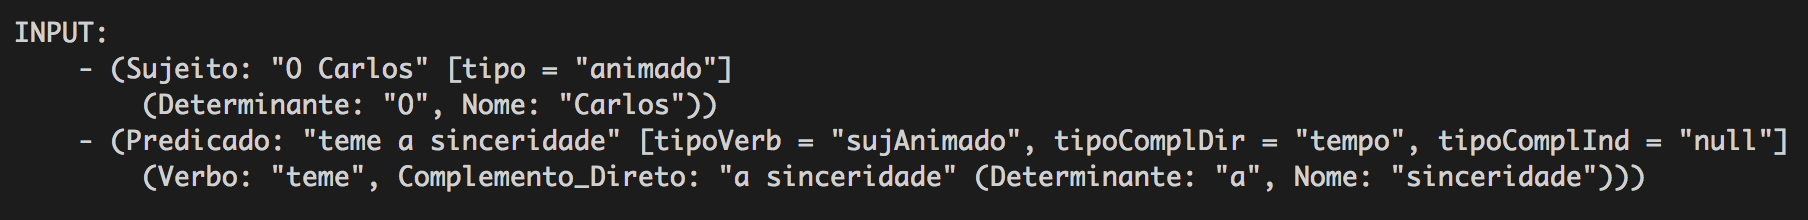
\includegraphics[width=15cm]{images/INPUT_meta_grammar_example.png}
    \caption{Example of the students parsing.}
    \label{fig:meta_grammar_student}
\end{figure}

\section{Case Study}
After the conception of a possible system architecture and DSL, the first task was to define the \textsc{DSL} that was supposed to be generated by the ``meta-language'' processor. This \textsc{DSL} would be the translation of the previously defined language into \textsc{ANTLR} instructions, that have as main purpose to verify the sentences written by the students. The \textsc{DSL} design consists in slicing the sentence into main parts, with each main part possibly having more parts into them. These parts are supposed to be specified by the teacher, but in this context, as a case study, it was assumed that a structure is predefined.

\subsection{Attribute Validation}
This case study intends to validate sentence components based on their attributes, where certain components require certain types of attributes in different components of the sentence. The example shows that one sentence is divided into two main parts: a subject (\underline{sujeito}) and a predicate (\underline{predicado}). The subject is then subdivided into a possible pronoun (\underline{pronome}) and a noun (\underline{nome}), which are then matched with a word (in this example the words are predefined). The predicate is composed by the verb (\underline{verbo}) and two complements that are directly and indirectly (\underline{complementoDireto} and \underline{complementoIndireto}) connected to the verb. Both these complements are composed by a possible pronoun or determinant (\underline{determinante}) followed by a quantifier (\underline{quantificador}) and a noun. The verb is, like the noun, predefined.

% Excerto da DSL para caso de estudo.
\begin{figure}[h]
    \centering
    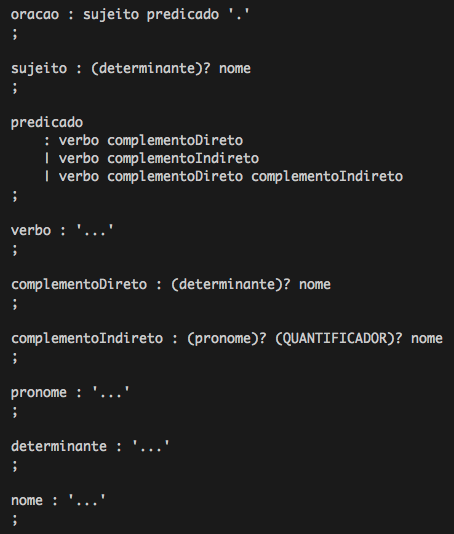
\includegraphics[width=12cm]{images/dsl_excerpt.png}
    \caption{Example DSL excerpt.}
    \label{fig:dsl_excerpt}
\end{figure}

All that is left to do, is to start evaluating all the different attributes that each component has, and to check if the sentence provided by the student is, according to the rules, valid. 

As shown in the excerpt below, and based on different set of attributes and rules, if the verb requires an \textbf{animated} subject then if the subject is \textbf{inanimated} an error message should appear, and notify the student of that same error. These error messages are the translation of the ``ERRORS'' block explained on the previous section.

% Excerto da validação de atributos na gramática.
\begin{figure}[h]
    \centering
    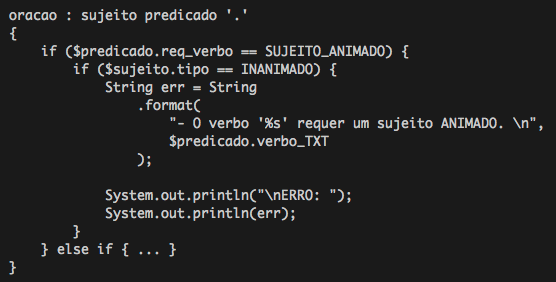
\includegraphics[width=12cm]{images/dsl_validation.png}
    \caption{Example DSL attribute validation.}
    \label{fig:dsl_attribute_validation}
\end{figure}

To conclude, if we use as an input a sentence like
\begin{description}
    O Carlos teme a sinceridade.
\end{description}
the sentence is accepted because, firstly, the structure is correct, and every component is in the right place, and secondly, all the attributes obey to the rules. As another example, if we use as an input other sentence for example \begin{description}
    O acidente teme a sinceridade.
\end{description}
we get an error which indicates that the verb ``teme" requires an animated subject, and ``acidente'' belongs to the subject that has an inanimated property.

% Exemplo de um erro na dsl de teste.
\begin{figure}[h]
    \centering
    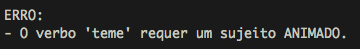
\includegraphics[width=10cm]{images/animated_subject_error.png}
    \caption{Example of an error message.}
    \label{fig:error_message_dsl}
\end{figure}

\subsection{Number and Gender}
This case study, based on the same \textsc{DSL} excerpt [\ref{fig:dsl_excerpt}], intends to validade the gender and number within the subject. Two of the productions, \textbf{determinante} and \textbf{nome}, need to be in concordance when it comes to gender and number. By using synthesized attributes, we can return the genders and numbers of the given words.

% produção do determinante dsl excerpt
\begin{figure}[h]
    \centering
    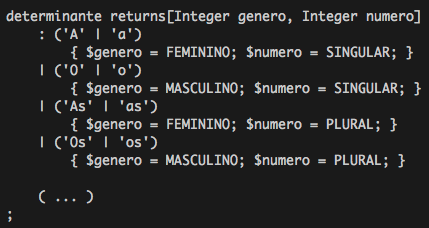
\includegraphics[width=10cm]{images/dsl_determinante_excerpt.png}
    \caption{Excerpt of the 'determinante' production.}
    \label{fig:determinante_dsl_excerpt}
\end{figure}

% produção do nome dsl excerpt
\begin{figure}[h]
    \centering
    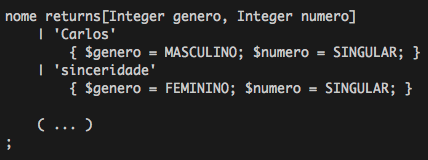
\includegraphics[width=10cm]{images/dsl_nome_excerpt.png}
    \caption{Excerpt of the 'nome' production.}
    \label{fig:nome_dsl_excerpt}
\end{figure}

Within the \textbf{sujeito} production, we can perform these two evaluations, and check if the sentence provided by the student is, again, according to the rules, valid.

% produção do sujeito dsl excerpt
\begin{figure}[h]
    \centering
    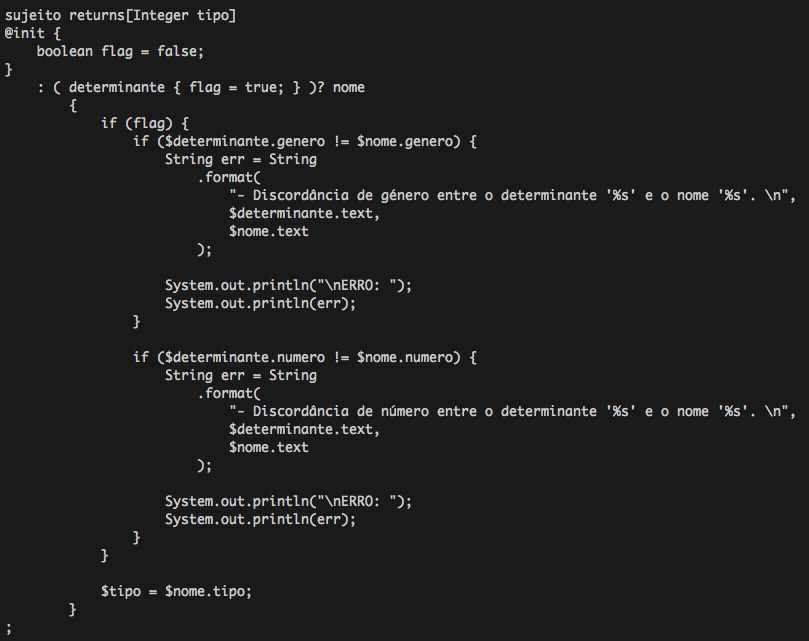
\includegraphics[width=13cm]{images/dsl_GenderNumber_validation.png}
    \caption{Example of gender/number validation within the 'sujeito' production.}
    \label{fig:sujeito_dsl_excerpt}
\end{figure}

To conclude this case study, if we use a similar input, but with an error
\begin{description}
    A Carlos teme a sinceridade.
\end{description}
we get a message indicating that the determinant and noun have a different gender.

% erro gender dsl excerpt
\begin{figure}[h]
    \centering
    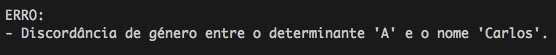
\includegraphics[width=11cm]{images/dsl_gender_error.png}
    \caption{Example of a gender error message.}
    \label{fig:erro_gender_dsl_excerpt}
\end{figure}

\noindent Using another input, for example
\begin{description}
    Os Carlos teme a sinceridade.
\end{description}
we can see that the gender matches, but the number in incorrect. Likewise, we get an error.

% erro number dsl excerpt
\begin{figure}[h]
    \centering
    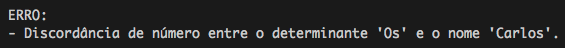
\includegraphics[width=11cm]{images/dsl_number_error.png}
    \caption{Example of a number error message.}
    \label{fig:erro_number_dsl_excerpt}
\end{figure}
\chapter{System Development} \label{system_development}

This section will present the development and workflow of the system. 
As previously mentioned, the next step was to expand the defined DSL, and to use attributes as a form of calculation. 
Most of the productions were expanded, allowing for certain calculations to be injected over the tree.

\section{Meta-Grammar}

With the grammar divided into 3 main parts (STRUCTURE, ERRORS, INPUT), different types of calculations occur at different sections. The STRUCTURE and ERRORS blocks are written in a single file (by the teacher) which is then joined 
with the INPUT block (written by the student). The process starts with searching for the teacher and student specification, and then compiling the program using a meta-grammar based processor. A new processor is generated to be 
used by the student to verify if his sentences are correctly following the structure defined by the teacher.

Within the grammar itself, the first rule
\newpage

%\begin{center}
%\begin{minipage}{11cm}
%\begin{Verbatim}[frame=single, framesep=2mm, fontsize=\small]
%determinante returns[Integer genero, Integer numero]
%    : ('A' | 'a')
%        { $genero = FEMININO; $numero = SINGULAR; }
%    | ('O' | 'o')
%        { $genero = MASCULINO; $numero = SINGULAR; }
%    | ('As' | 'as')
%        { $genero = FEMININO; $numero = PLURAL; }
%    | ('Os' | 'os')
%        { $genero = MASCULINO; $numero = PLURAL; }
%
%    (...)
%;
%\end{Verbatim}
%\end{minipage}
%\end{center}

\begin{center}
\begin{minipage}{11cm}
\begin{lstlisting}[language=java, basicstyle=\small, label={lst:processor}, caption=Processor rule from the meta-grammar]
processor
@init {
    /* Main data structure. */
    List<RoseTree> struct = new ArrayList<>();

    (...)
}
    : structure[struct]
      errors[struct]
      input[struct]
    {
        (...)
    }
\end{lstlisting}
\end{minipage}
\end{center}

\noindent starts by initializing the main data structure. This structure is responsible for storing all the information that is being parsed from the file given as input (the meta-language file). 

When choosing the correct structure to store all the important data, the first \/\*approach\*\/ taken was to store all components in a single Map, with each name of a component
matching their respective value. The problem with this approach, which was identified right away, was that is possible to exist two or more components with the same exact
name, causing a conflict within the Map. Furthermore, components have different information associated, like attributes, and it would be better if it is all in the same
place - this created the need for a Component class.

The Component class would store the name of the component, a possible value and a Map that associated each attribute with some value. The components would all be stored
within a List.
\newpage

\begin{center}
\begin{minipage}{10cm}
\begin{lstlisting}[language=java, basicstyle=\small, label={lst:component_class}, caption=Component class]
@members {
    class Component {
        String name;
        String lexical_part;
        Map<String, String> attributes;
    }

    /* Main data structure. */
    List<Component> struct;
}
\end{lstlisting}
\end{minipage}
\end{center}

The problem with this solution is that it does not follow any particular order (in this case, the STRUCTURE order), which can be very useful when validating the students
input, checking if it obeys to the structure previously defined.

The structure of the sentence takes a form of a tree, so that would be the correct way to store the information and maintain order. As each node could have less or more 
than two children, a binary tree was not the way to go. The idea was to build a Graph structure that used a mapped each node to a list of nodes.

\begin{center}
\begin{minipage}{11cm}
\begin{lstlisting}[language=java, basicstyle=\small, label={lst:graph_class}, caption=Graph class]
@members {
    class Graph
    {
        Map<Component, List<Component>> map;
    }
}
\end{lstlisting}
\end{minipage}
\end{center}

Although this could maintaing the order, the initial problem remainded. We could have components with the same exact properties, and this would cause conflict between
edges, and not create a new node when it was supposed to.

The principle of having a tree as the main data structure falls into the need of maintaining a valid path. For example, if the teacher says that the structure will have a component \emph{\textbf{A}}, and this component has two children, \emph{\textbf{B}} and \emph{\textbf{C}}, then the paths \emph{\textbf{A$\rightarrow$B}} and \emph{\textbf{A$\rightarrow$C}} should be stored. In this particular problem, it is required to have a tree that within each node has a list of children with an arbitrary size of \emph{\textbf{N}}.

Some backtracking was made to come up with an ideal solution. The prerequisites were that order needed to be maintained and each node (component) had an arbitrary number
of \emph{\textbf{N}} children. The previously created Component class would store all its values and a list of new components (children), creating a path between 
the parent component and said children. This type of structure is denominated as Rose Tree, which is a prevelant structure in the functional programming community. 
It is a multi-way tree, with an unbounded number of branches per node. This way, all the prerequisites would be matched, and all the information correctly stored. 

\begin{center}
\begin{minipage}{9cm}
\begin{lstlisting}[language=java, basicstyle=\small, label={lst:rosetree_class}, caption=RoseTree class]
class RoseTree {
    String value;
    boolean required;
    Map<String, String> attributes;
    List<String> lexical_part;
    List<RoseTree> children;

    (...)
}
\end{lstlisting}
\end{minipage}
\end{center}

When in the main production (\emph{processor}), a list of \emph{Rose Trees} is initialized, with each tree of the list corresponding to the main components of the sentence. This structure would travel along the parsing tree, to first be populated with information and then serving as the main source of validation and checking.

On the first block (STRUCTURE) there are not many calculations happening within the productions. 
The main task is to simply validate the syntax and extract data to be stored in the \emph{Rose Tree}. 
For each node, it is stored the name of the component, if it is required to be declared or not, a group of attributes (could be non-existent), 
a lexical part (if it is the case), and finally a list of nodes, referred as the children.

After the parsing of the structure, there are a list of conditions named ERRORS that need to be validated and converted into \emph{Java} syntax - this conversion would then be injected on the main rule of the generated grammar. These logical expressions are based on the attributes of each component and their relations. For example, if the teacher says that a component \emph{\textbf{A}} has an attribute named \emph{\textbf{a}}, and this attribute is required to have value \emph{\textbf{x}}, if the student assigns it a value of \emph{\textbf{z}}, then an error should appear. All these conditions can be combined with the logical operands ``AND'' or ``OR''. The way that is parsed is based on the path specified by the teacher when accessing the attribute. Using the example before, a component \emph{\textbf{A}} with a child \emph{\textbf{B}}, with \emph{\textbf{B}} having a attribute \emph{\textbf{x}}, in order to access it the syntax should be

A.B -\textgreater x

\noindent as the full path is required. This is done in order to calculate the correct path and avoid ambiguity between attributes. Over the parsing of these rules, the path is being validated, and in case of any error, the user is notified.

Finally, the last block corresponds to the input that was written by the student. 
The goal is to validate the components that were defined, and match them with the structure created by the teacher. 
Again, the RoseTree was used as a way to check if the student’s components and paths were valid. 
The task of the student was to ``parse'' his sentence and divide it by components, identifying the lexical segments and storing them within a node of the \emph{Rose Tree}. 
At last, the main rule of the Meta-Grammar makes use of a generator to generate all the rules for the Specific Natural Language Grammar. 
Within this generator, the various \emph{Rose Tree's} are passed as an argument and then traversed recursively.
% In the case of any error, the user is informed of where the error happened but also in which component. 
% Furthermore, when parsing attributes and their respective values, if the student defines two attributes with the same name, but with different values, 
% a warning is raised to inform the user that the value that was considered was the last one to be recognized.

\section{Meta-Language Processor}

In order to simplify the usage of the Meta-Grammar, and as the grammar itself made use of auxiliar \emph{Java} classes, all of that was combined into a \emph{JAR} file.
Having this type of package would allow for a more flexible integration with any component.
The Meta-Language Processor, which was created by providing the Meta-Grammar file to ANTLR, could now be used with the \emph{JAR} file, 
providing as input the Meta-Language Specification. 

Using the command line, the instruction:
\begin{Verbatim}
	java -jar lib/MetaGrammar.jar input/meta-lang
\end{Verbatim}
\noindent tries to generate the Specific Natural Language Grammar, based on the input provided. In case of any error, the grammar would not be generated.

\begin{figure}[h]
    \centering
    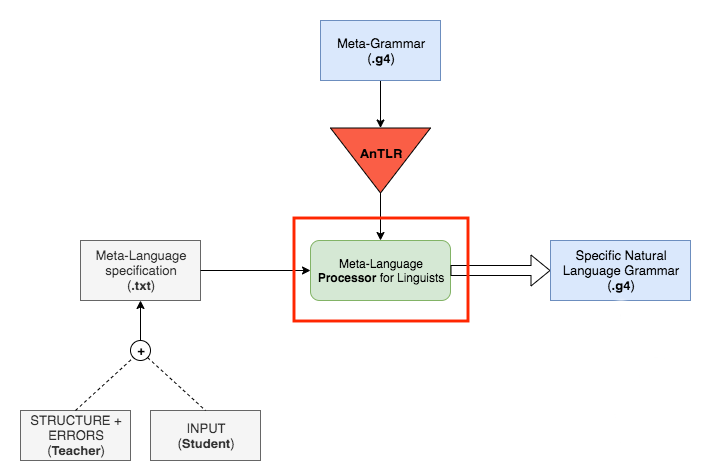
\includegraphics[width=10cm]{images/system_meta_processor.png}
    \caption{Excerpt of the system architecture.}
    \label{fig:system_architecture}
\end{figure}

\section{Sentence Validator}

If no errors occur in the previous step, we should now have a file named ``Grammar.g4" that corresponds to the Specific Natural Language Grammar.
This grammar contains all the tokens extracted from the Meta-Language specification, and combining it with ANTLR, we create a new specific Sentence Validator.
When providing the student's sentence to the Sentence Validator, and if all goes well, a Syntax Tree should be generated using a tool called \emph{TestRig}.
Using once again the command line, and providing a specific flag to the tool (-gui):
\begin{Verbatim}
	java -cp \ 
		"lib/antlr-4.8-complete.jar:$CLASSPATH" \ 
		org.antlr.v4.gui.TestRig \ 
			Grammar main input/sentence \ 
		-gui
\end{Verbatim}
\noindent we obtain the final syntax tree for the sentence provided. 
As an example, using \autoref{lst:metaStruct} and \autoref{lst:metaInput}, the generated syntax tree would be:

\begin{figure}[h]
    \centering
    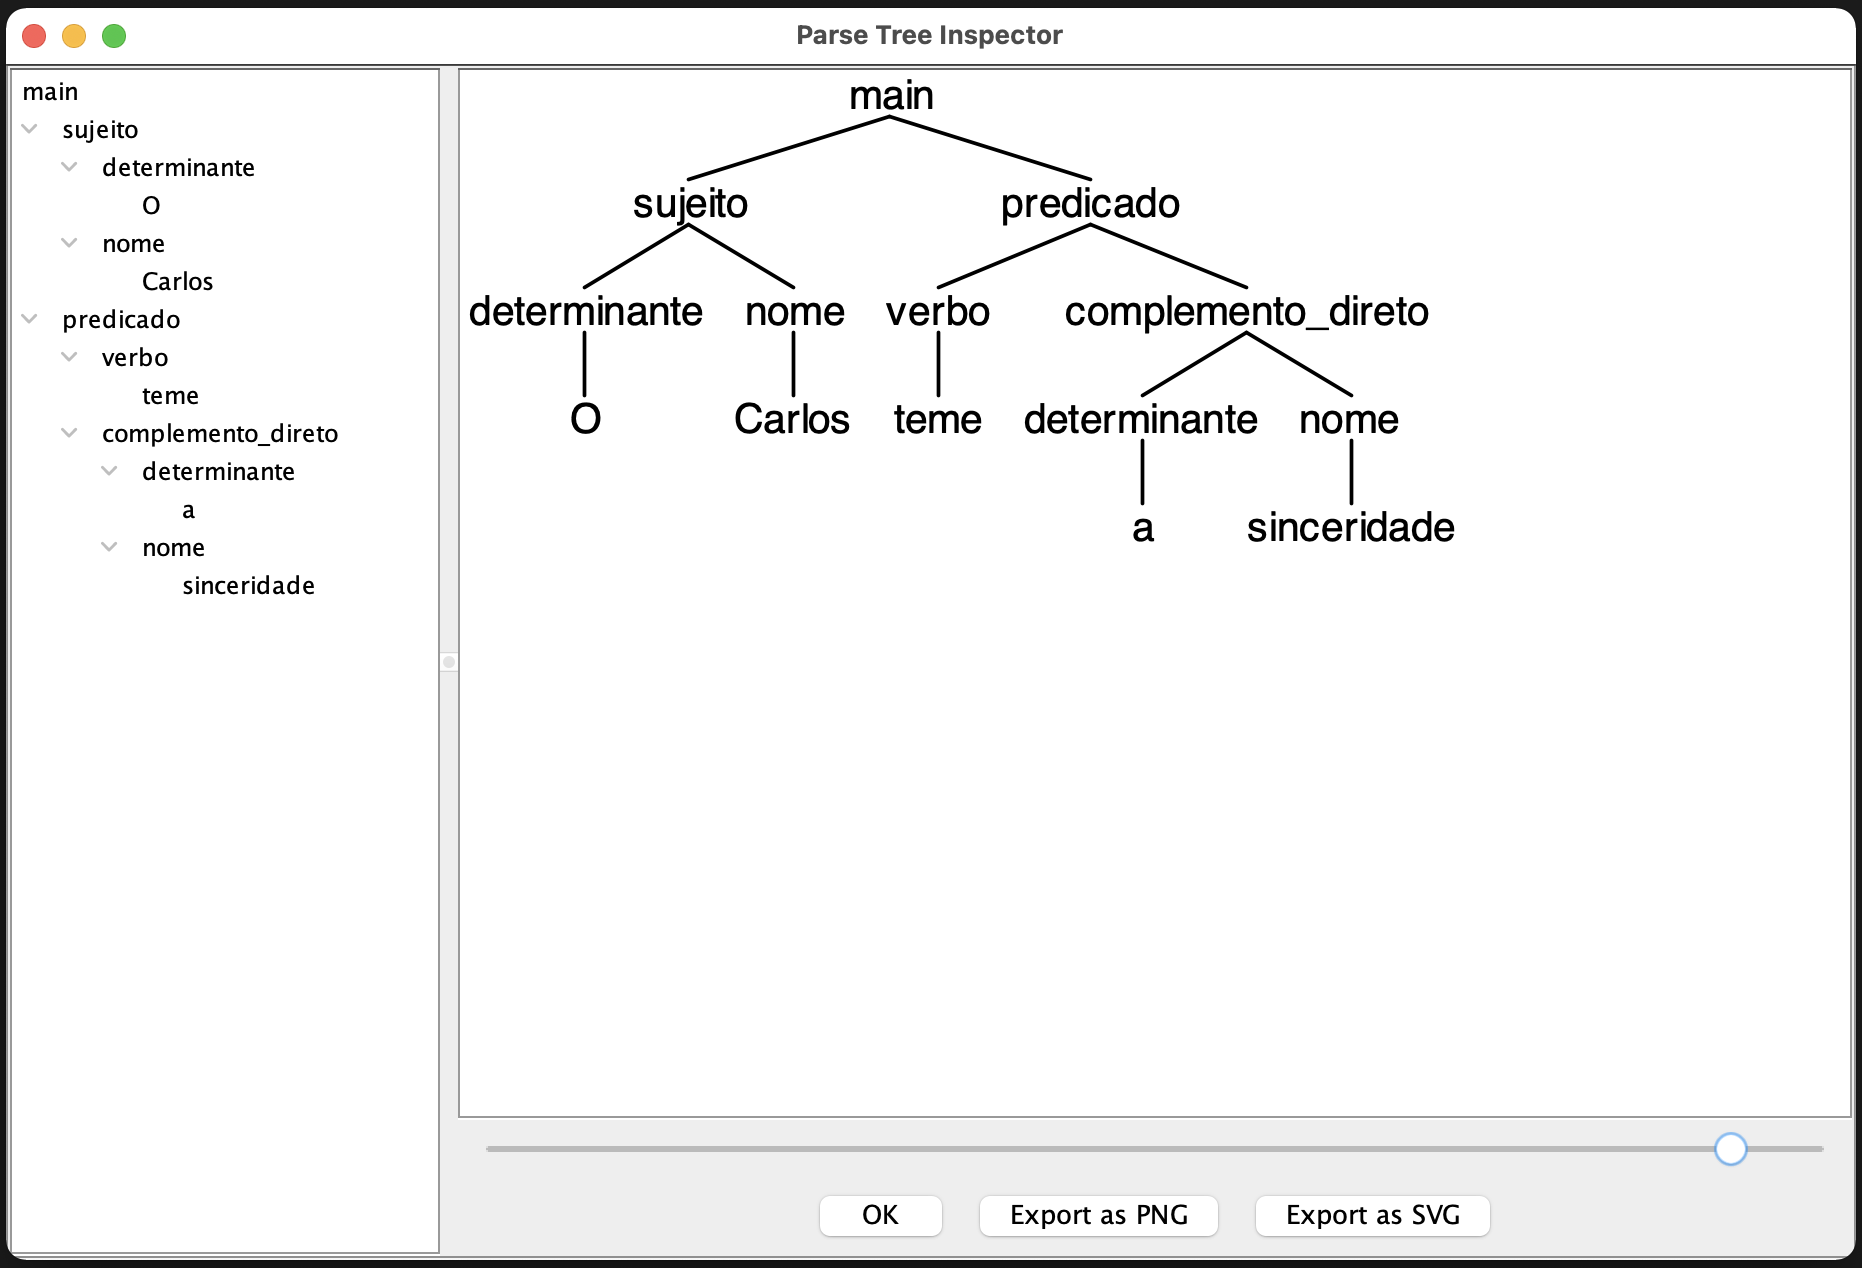
\includegraphics[width=10cm]{images/testrig_gui_example.png}
    \caption{Example of a generated syntax tree within TestRig.}
    \label{fig:system_architecture}
\end{figure}



% Having parsed the meta-language file, a generator is called by the main rule - the \emph{Rose Tree} is passed as an argument and then traversed in order to generate all 
% the rules for the Specific Natural Language Grammar.
% This grammar, after being generated, is used to create a processor in which the student's sentence will be used as input, creating a visual 
% syntax tree of that same sentence.

\chapter{Case Studies} \label{case_study}
In order to better explain the solution architecture presented in this thesis, some concrete examples will be presented in this section. 
The main idea is to show the specifications used by the teacher and by the student and how the generator processor verifies the correcteness of the student sentences. 
The DSL design consists in slicing the sentence into parts, and each part can have subparts.

\textbf{Lyntax}, the word that combines the terms ``Linguistics" and ``Syntax", was the name chosen for a system that combines both the meta-language processor and
the user interface that makes use of such processor.
These case studies are also relevant as an example for a possible pedagogical scenario by using the system in a classroom context.
The purpose of this chapter is to also demonstrate some of the process in which both the Teacher and Student will be involved, and to exhibit some common structures
and inputs as well as their results.

\section{Attribute Validation}
This case study intends to demonstrate the validation on sentence components based on their attributes. The example showed in the previous chapter 
\autoref{lst:metaStruct} contains a structure that is composed by two main parts: a subject (\underline{Sujeito}) and a predicate (\underline{Predicado}). 
The subject is then subdivided into a possible determiner (\underline{Determinante}) and a noun (\underline{Nome}), which are then matched with a word 
(the lexical part identified by the student). The predicate is composed by a verb and a complement that is directly related to the verb. This complement 
(\underline{Complemento\_Direto}) is then composed by a possible determiner (\underline{Determinante}) and a mandatory noun (\underline{Nome}).

In this particular example, both the subject and the verb from the predicate have an attribute named ‘tipo’ which purpose is to check evaluate if each of the components
are animated or inanimated. By analysing the logic in the ERRORS block \autoref{lst:metaStruct}, we can see that if the value of the attribute ‘tipo’ is different 
between the two components, than an error should be pointed. In this case, the sentence parsed by the student is

``O Carlos teme a sinceridade.''

\noindent which is in fact a valid sentence, as the name ``Carlos'' and the verb ``teme'' are both animated.

When running the example above (\autoref{lst:metaStruct} plus \autoref{lst:metaInput}) in the Meta Grammar processor, and if no errors occur, a specific grammar (in ANTLR) 
in then generated. For this specific case, this is the generated grammar.

\begin{center}
\begin{minipage}{15cm}
\begin{lstlisting}[language=java, basicstyle=\tiny, label={lst:case_study_sentence}, caption=Example of a specific generated grammar.]
grammar Grammar;

@members {
    final String Sujeito__TIPO = ``animado";
    final String Predicado__Verbo__TIPO = ``animado";
}


main : sujeito predicado
{
    if ( Sujeito__TIPO.equals(``animado") && Predicado__Verbo__TIPO.equals(``inanimado") ) 
        { System.out.println(``ERROR!"); }

    if ( Sujeito__TIPO.equals(``inanimado") && Predicado__Verbo__TIPO.equals(``animado") ) 
        { System.out.println(``ERROR!"); }
}
;

sujeito : (determinante)? nome 
;

determinante : 'O' | 'a'
;

nome : 'Carlos' | 'sinceridade'
;

predicado : verbo complemento_direto 
;

complemento_direto : (determinante)? nome 
;

verbo : 'teme'
;


/* LEXER */
(...)
\end{lstlisting}
\end{minipage}
\end{center}

In the ‘main’ production, we can see the logical conditions that are ready to be evaluated when running this grammar. As the conditions are false, no errors should occur,
allowing for the visualization of the syntax tree.

% INSERIR PRINT DO TESTRIG????

%To conclude, if we use as an input a sentence like
%
%``O Carlos teme a sinceridade.''
%
%\noindent the sentence is accepted because, firstly, the structure is correct, and every component is in the right place, and secondly, all the attributes obey to the rules. As another example, if we use as an input other sentence for example
%
%``O acidente teme a sinceridade.''
%
%\noindent we get an error which indicates that the verb ``teme'' requires an animated subject, and ``acidente'' belongs to the subject that has an inanimated property.
%
%\begin{center}
%\begin{minipage}{10cm}
%\begin{lstlisting}[language=java, basicstyle=\small, label={lst:error_message_dsl}, caption=Example of an error message]
%ERRO:
%- O verbo 'teme' requer um sujeito ANIMADO.
%\end{lstlisting}
%\end{minipage}
%\end{center}

\section{Missing components \& Warnings}
Still based on the previous defined structure \autoref{lst:metaStruct}, the student's specification can still be missing some components that are mandatory. 
This case study just intends to show the way that errors or warnings are notified to the user.

In order to demonstrate this, the input block defined above \autoref{lst:metaInput} is going to suffer some modifications in order to trigger errors or warnings.

\begin{center}
\begin{minipage}{13cm}
\begin{lstlisting}[language=java, basicstyle=\small, label={lst:meta_input_missing_comp}, caption=Example of the students parsing with missing component]
INPUT:
    - (Sujeito: ``O Carlos" [tipo = ``animado"]
        (Determinante: ``O"))
    - (Predicado: ``teme a sinceridade" 
        (Verbo: ``teme" [tipo = ``animado"], 
         Complemento_Direto: ``a sinceridade" 
            (Determinante: ``a", Nome: ``sinceridade")))
\end{lstlisting}
\end{minipage}
\end{center}

In this example, we can see that within the subject component (\underline{Sujeito}), the noun component (\underline{Nome}) is not defined. 
This particular case would cause an error as the noun component is mandatory (based on the previous structure \autoref{lst:metaStruct}). 
The error message identifies the missing component.

\begin{center}
\begin{minipage}{13cm}
\begin{lstlisting}[language=java, basicstyle=\small, label={lst:err_msg_missing_comp}, caption=Example error message of missing component]
ERROR: (INPUT) 
- The mandatory component 'Nome' has not been defined.
\end{lstlisting}
\end{minipage}
\end{center}
Another possible error would be to not define attributes, and to not give those attributes values. In this case, if we remove the attribute ‘tipo’ from the subject 
component (\underline{Sujeito}),

\begin{center}
\begin{minipage}{13cm}
\begin{lstlisting}[language=java, basicstyle=\small, label={lst:meta_input_missing_attr}, caption=Example of the students parsing with missing attribute]
INPUT:
    - (Sujeito: ``O Carlos"
        (Determinante: ``O", Nome: ``Carlos"))
    - (Predicado: ``teme a sinceridade" 
        (Verbo: ``teme" [tipo = ``animado"], 
         Complemento_Direto: ``a sinceridade" 
            (Determinante: ``a", Nome: ``sinceridade")))
\end{lstlisting}
\end{minipage}
\end{center}

\noindent the error should notify the user that the subject component is missing attributes, as attributes are always mandatory (if the component related to them is also
mandatory).

\begin{center}
\begin{minipage}{14cm}
\begin{lstlisting}[language=java, basicstyle=\small, label={lst:err_msg_missing_attr}, caption=Example error message of missing attributes]
ERROR: (INPUT)
- There are attributes related to the component 'Sujeito' that were not defined.
\end{lstlisting}
\end{minipage}
\end{center}

When it comes to warnings, there is only one case that raises them. This happens when the user defines the same attribute multiple times, warning that only the last value 
will be considered for the final evaluation. If, for example, we use the same attribute twice on the subject component,

\begin{center}
\begin{minipage}{14cm}
\begin{lstlisting}[language=java, basicstyle=\small, label={lst:meta_input_attr_twice}, caption=Example of the students parsing with the same attribute in a single component]
INPUT:
    - (Sujeito: ``O Carlos" 
        [tipo = ``animado", tipo = ``inanimado"]
        (Determinante: ``O", Nome: ``Carlos"))
    - (Predicado: ``teme a sinceridade" 
        (Verbo: ``teme" [tipo = ``animado"], 
         Complemento_Direto: ``a sinceridade" 
            (Determinante: ``a", Nome: ``sinceridade")))
\end{lstlisting}
\end{minipage}
\end{center}

\noindent a warning is raised to notify the user that only the last value was considered as final (\emph{tipo = ``inanimado''}).

\begin{center}
\begin{minipage}{14cm}
\begin{lstlisting}[language=java, basicstyle=\small, label={lst:meta_input_missing_attr_warn}, caption=Example warning message of same attribute in a single component]
WARNING: (INPUT) 
- The attribute 'tipo' has already been declared! Using the last value found.
\end{lstlisting}
\end{minipage}
\end{center}

\section{Arbitrary Structure}

This last case study has the intention to demonstrate that is possible to define any arbitrary sentence structure, without obeying to any specific linguistic rules. If, for instance, the main goal of the teacher is to test
different attributes despite of the components of a sentence, a simple structure can be defined for that same purpose. The following structure and rules intend to test the gender between two components, and this can be done 
with very simple sentences.

\begin{center}
\begin{minipage}{15cm}
\begin{lstlisting}[language=java, basicstyle=\tiny, label={lst:arbitrary_structure}, caption=Example of an arbitrary sentence structure]
STRUCTURE:
    part(
        Frase,
        subparts[
            (Determinante, attributes{genero}),
            (Nome, attributes{genero}),
            (Verbo)
        ]
    )

ERRORS:
    Frase.Determinante->genero = ``masculino" AND Frase.Nome->genero = ``feminino";
    Frase.Determinante->genero = ``feminino" AND Frase.Nome->genero = ``masculino";
    
    Frase.Determinante->genero != ``masculino" AND Frase.Determinante->genero != ``feminino";
    Frase.Nome->genero != ``masculino" AND Frase.Nome->genero != ``feminino";
\end{lstlisting}
\end{minipage}
\end{center}

Based on the rules written, we can see that the gender must be equal, or the sentence is invalid. Furthermore, the rules ensure that the gender can only be male or female (``masculino'' and ``feminino'' respectively) in order
to be a valid sentence.

\begin{center}
\begin{minipage}{14cm}
\begin{lstlisting}[language=java, basicstyle=\tiny, label={lst:arbitrary_structure_input}, caption=Example of an arbitrary sentence input]
INPUT:
    - (Frase: ``A Olinda come"
        (Determinante: ``A" [genero = ``feminino"],
         Nome: ``Olinda" [genero = ``feminino"],
         Verbo: ``come"))
\end{lstlisting}
\end{minipage}
\end{center}

Combining all the information in the processor, we generate a specific grammar for this arbitrary structure.

\begin{center}
\begin{minipage}{15cm}
\begin{lstlisting}[language=java, basicstyle=\tiny, label={lst:case_study_sentence}, caption=Example of a specific generated grammar.]
grammar Grammar;

@members {
    final String Frase__Determinante__GENERO = ``feminino";
    final String Frase__Nome__GENERO = ``feminino";
}


main : frase
{
    if ( Frase__Determinante__GENERO.equals(``masculino") && Frase__Nome__GENERO.equals(``feminino") ) 
        { System.out.println(``ERROR!"); }
	
    if ( Frase__Determinante__GENERO.equals(``feminino") && Frase__Nome__GENERO.equals(``masculino") ) 
        { System.out.println(``ERROR!"); }
	
    if ( !Frase__Determinante__GENERO.equals(``masculino") && !Frase__Determinante__GENERO.equals(``feminino") ) 
        { System.out.println(``ERROR!"); }
	
    if ( !Frase__Nome__GENERO.equals(``masculino") && !Frase__Nome__GENERO.equals(``feminino") ) 
        { System.out.println(``ERROR!"); }
}
;

frase : determinante nome verbo 
;

determinante : 'A'
;

nome : 'Olinda'
;

verbo : 'come'
;


/* LEXER */
(...)
\end{lstlisting}
\end{minipage}
\end{center}


This simple example shows that the meta-language created is flexible to the point of writing arbitrary sentences or rules, 
augmenting the possibilities of syntactic structures.

\section{Further examples and structures}

In order to demonstrate even further the capabilities of the tool, some more examples of simple (but concrete) and complex sentences will be included.
Some of the previous examples had the intent of demonstrating validations and/or trigger errors and warnings.
These next examples intend to explore more common tested structures and structures a bit more complex.

This first example is, again, composed by a Subject - Predicate structure, with some caracteristics to the Predicate itself.

\begin{center}
\begin{minipage}{14cm}
\begin{lstlisting}[language=java, basicstyle=\small, label={lst:example_structure1}, caption=Example of a sentence structure]
STRUCTURE:
    part[(Sujeito)]
    part[(
        Predicado,
        subparts[
            (Verbo),
            (Complemento_Direto),
            (Predicativo_Complemento_Direto)?
        ]
    )]
\end{lstlisting}
\end{minipage}
\end{center}

\begin{center}
\begin{minipage}{14cm}
\begin{lstlisting}[language=java, basicstyle=\small, label={lst:example_input1}, caption=Example of a sentence input]
INPUT:
    - (Sujeito: ``O rapaz")

    - (Predicado (
        Verbo: ``viu",
        Complemento_Direto: ``o homem",
        Predicativo_Complemento_Direto: ``com o telescopio"
    ))
\end{lstlisting}
\end{minipage}
\end{center}


The next example uses an attribute to limit the domain of a component (\textit{Complemento\_Circunstancial}).

\begin{center}
\begin{minipage}{15cm}
\begin{lstlisting}[language=java, basicstyle=\small, label={lst:example_structure3}, caption=Example of a sentence structure]
STRUCTURE:
    part[(
        Frase, subparts[
            (Modificador),
            (Sujeito),
            (Predicado, subparts[
                (Verbo),
                (Complemento_Direto),
                (Complemento_Circunstancial, attributes{tipo})
            ])
        ]
    )]

ERRORS:
    Frase.Predicado.Complemento_Circunstancial->tipo != ``lugar";
\end{lstlisting}
\end{minipage}
\end{center}

\begin{center}
\begin{minipage}{15cm}
\begin{lstlisting}[language=java, basicstyle=\small, label={lst:example_input3}, caption=Example of a sentence input]
INPUT:
    - (Frase (
        Modificador: ``Hoje",
        Sujeito: ``eu",
        Predicado (
            Verbo: ``comi",
            Complemento_Direto: ``uma pizza",
            Complemento_Circunstancial: "na pizzaria abaixo" [tipo = ``lugar"]
        )
    ))
\end{lstlisting}
\end{minipage}
\end{center}


We can also use an ``\emph{\(|\)}" (\textit{or}) operator within the structure rules, giving the student the possibility of defining one or other component,
but maintaing the main structure of the sentence. 
Using an operator with this capability, we prevent the need of creating two separate structures only for a single change. 

\begin{center}
\begin{minipage}{10cm}
\begin{lstlisting}[language=java, basicstyle=\small, label={lst:example_structure4}, caption=Example of a sentence structure]
STRUCTURE:
    part[(
        Frase, subparts[
            (Interjeccion | Pronombre),
            (Verbo),
            (Nombre)
        ]
    )]
\end{lstlisting}
\end{minipage}
\end{center}

\begin{center}
\begin{minipage}{10cm}
\begin{lstlisting}[language=java, basicstyle=\small, label={lst:example_input4}, caption=Example of a sentence input]
INPUT:
    - (Frase (
        Interjeccion: ``Hola!",
        Verbo: ``Soy",
        Nombre: ``Manuel"
    ))
\end{lstlisting}
\end{minipage}
\end{center}


Below is an example of a complex structure which supports more complex sentences.
In this particular case we are using two predicates (\textit{Predicado}), both joined by a conjunction (\textit{Conjuncao}).
This example intends to demonstrate the capability of the tool when it comes to even bigger and complex structures.
The principal remains the same, it all depends on the rules defined by the teacher.

\begin{center}
\begin{minipage}{12cm}
\begin{lstlisting}[language=java, basicstyle=\small, label={lst:example_complex_structure}, caption=Example of a complex sentence structure]
STRUCTURE:
    part[(Sujeito)]
    part[(
        Predicado,
        subparts[
            (Verbo),
            (Complemento_Indireto)
        ])
    )]
    part[(Conjuncao)]
	part[(
        Predicado,
        subparts[
            (Verbo),
            (Modificador_Verbal)
        ]
    )]
\end{lstlisting}
\end{minipage}
\end{center}


\begin{center}
\begin{minipage}{12cm}
\begin{lstlisting}[language=java, basicstyle=\small, label={lst:example_complex_input}, caption=Example of a complex sentence input]
INPUT:
    - (Sujeito: ``Los soldados")

    - (Predicado (
        Verbo: ``dispararam",
        Complemento_Indireto: ``a los sentenciados"
    ))

    - (Conjuncao: ``y")

    - (Predicado (
        Verbo: ``cayeron",
        Modificador_Verbal: ``muertos"
    ))
\end{lstlisting}
\end{minipage}
\end{center}

Other example...

\begin{center}
\begin{minipage}{13cm}
\begin{lstlisting}[language=java, basicstyle=\small, label={lst:example_complex_structure2}, caption=Example of a complex sentence structure]
STRUCTURE:
    part[(Sujeito)]
    part[(
        Predicado,
        subparts[
            (Verbo),
            (Complemento_Circunstancial_Lugar)
        ])
    )]
    part[(Conjuncao)]
    part[(Sujeito)]
	part[(
        Predicado,
        subparts[
            (Verbo),
            (Complemento_Circunstancial_Lugar)
        ]
    )]
\end{lstlisting}
\end{minipage}
\end{center}


\begin{center}
\begin{minipage}{13cm}
\begin{lstlisting}[language=java, basicstyle=\small, label={lst:example_complex_input22}, caption=Example of a complex sentence input]
INPUT:
    - (Sujeito: ``Juan")

    - (Predicado (
        Verbo: ``vive",
        Complemento_Indireto: ``en el edificio blanco"
    ))

    - (Conjuncao: ``y")

    - (Sujeito: ``Maria")

    - (Predicado (
        Verbo: ``trabaja",
        Complemento_Circunstancial_Lugar: ``aqui"
    ))
\end{lstlisting}
\end{minipage}
\end{center}

\chapter{Conclusion} \label{conclusion}

With this document, the main objective was to conduct a study and analysis about what this problem involves and what could, in any way, help create an adequate solution. Furthermore, the first approach to the problem was documented, giving special attention to the case studies and a first sketch of what will become a new language for linguists.

Regarding to the approaches that were taken, it is quite clear that some parts are still at an early stage of development, and require more time - mainly the design of the students \textsc{DSL}, which is still very verbose in comparison to what was projected. The next step, which was already taken, is the creation of the meta-grammar that processes the information written by the teacher + student, and generates the \textsc{ANTLR} instructions based on the defined structure. The generated grammar will be based on the \textsc{DSL} structure that was used for the case studies. Afterwards, with a functional validator, the goal is to build a system with a user interface that allows to visualize the syntax tree of the input sentence, helping when it comes to analyse each segment individually.

\section{Working Plan}
The outlined work plan for this master thesis will consist of six phases. Each phase will include the conclusions of the previous phases and build upon the knowledge gained in each one.

\begin{description}
	\item[Phase 1] Bibliographic search in applying attribute grammars to linguistics, and study the tools that are already available.
	\item[Phase 2] Design the domain specific language (\textsc{DSL}) with all the requeriments previously mentioned.
	\item[Phase 3] Create the language translator in \textsc{ANTLR}.
	\item[Phase 4] Create the user interface.
	\item[Phase 5] Test and required adjustments.
	\item[Phase 6] Write Thesis.
\end{description}

For a better visualization, it was created a diagram based on all the different phases, divided into the months.

\begin{table}[!ht]
\centering
\caption{Activities Plan detailed}
\vspace{0.2cm}
\label{roadmap}
\scalebox{0.5}{
\def\S{\cellcolor{gray!75}}
\begin{tabular}{cp{0.5\linewidth}:cccc:cccc:cccc:cccc:cccc:}
\hline
\cline{1-14} % linha entre os anos e meses
Phase & Phase Description & Sep & Oct & Nov & Dec & Jan & Feb & Mar & Apr  & May & Jun & Jul & Aug \\
\hline
1& Bibliographic search & \S & \S & & &  &  &  &  &  &  &  & &   \\[4ex] % entre & & é o conteúdo da coluna
\\[0.5ex] % espaço em branco entre linhas
2& Designing the \textsc{DSL} & & & \S & \S & &  &  &  &  & & & \\[4ex]
\\[0.5ex]
3& Creating the language translator\ & & & & & \S & \S & \S & \\[4ex]
\\[0.5ex]
4& Creating the user interface. &  &  &  &  & & & & \S & \S &  &  & \\[4ex]
\\[0.5ex]
5& Testing and adjustments &  &  &  &  &  & & & & & \S & & & \\[4ex]
\\[0.5ex]
6& Finishing writing the thesis &  &  &  &  &  &  &  &  &  & & \S & \S & \\[4ex]
\end{tabular} }
\end{table}
%\chapter*{Bibliography}       

% % BIBLIOGRAPHY

%\newpage
\addcontentsline{toc}{chapter}{Bibliography}
\bibliographystyle{apalike}
\bibliography{lib}

\end{document}
